\chapter{Résultats}
Les expériences ont été réalisés avec Xvfb.

\section{Expérience 1 : étude à long terme}
\subsection{Détails de l'expérience}
Le but de cette expérience est de déterminer l'évolution des trackers sur une certaine période en effectuant des mesures de façon régulière.

Afin de réaliser cette étude, le \textit{crawler} a été lancé chaque jour du 28 mars au 7 mai 2014 (à l'exception du 8 avril) sur le TOP 1000 du classement Alexa \cite{AlexaTop}, ce qui représente 40 jours de mesures. Notez cependant que l'implémentation du compteur de cookies Flash a été réalisée ultérieurement à cette expérience et ces données ne sont donc pas disponibles au sein de l'expérience.
\newline

Le \textit{crawler} a été lancé avec les paramètres suivants :
\begin{itemize}
	\item les sites visités sont issus du TOP Alexa du 26 mars 2014
	\item l'intervalle sélectionné concerne les 1000 premiers sites
	\item 3 tentatives maximum ont été autorisées par site
	\item Firefox était redémarré tous les 50 sites
	\item Firefox était dépourvu de toute extension (autre que Firebug et NetExport)
	\newline
\end{itemize}

\subsection{Premières constatations}
Lors de cette expérience, on peut voir que le taux d'échec avec le \textit{crawler} est toujours inférieur à 9\%.
Notez que l'implémentation a un peu changé depuis cette expérience. Lors de cette dernière, quand un site atteignait le nombre maximum de tentatives et qu'il était placé dans la liste des sites en échec, il était également retiré de la liste des sites ayant eu besoin d'au moins un nouvel essai suite à un timeout.
Ceci explique des situations telles que sur la \autoref{Exp1_crawler_fails} au début du mois de mai.

\begin{figure}[h]
	\centering
	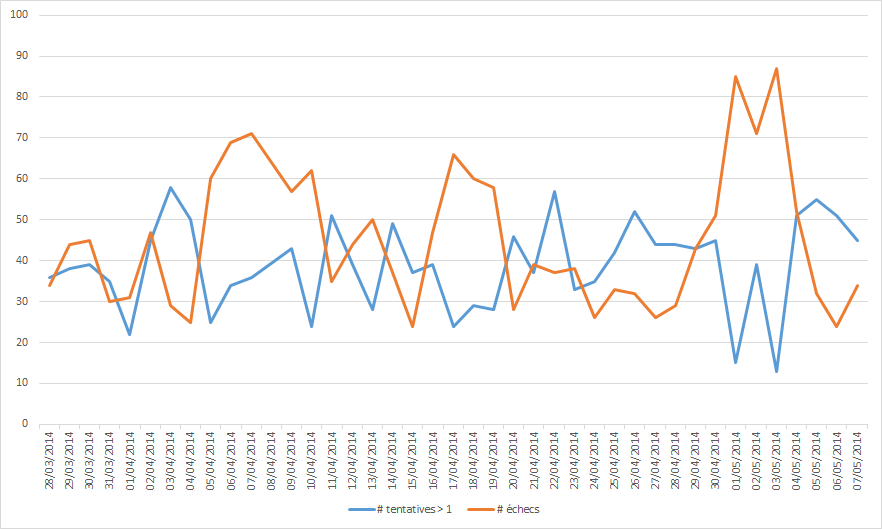
\includegraphics[scale=.7]{graphiques/Exp1_crawler_fails.png}
	\caption{\label{Exp1_crawler_fails}Le nombre d'échecs du \textit{crawler}}.
\end{figure}

\begin{figure}[h]
	\centering
	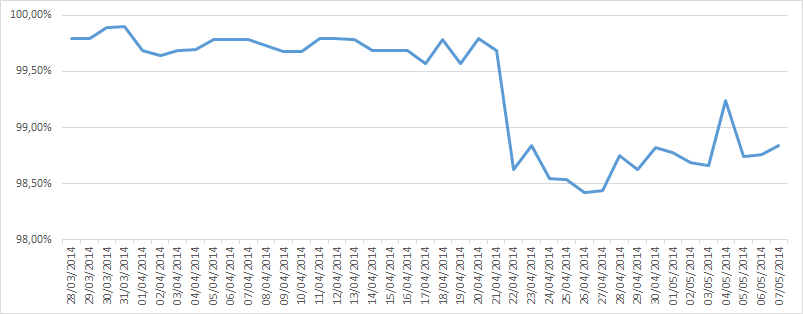
\includegraphics[scale=.8]{graphiques/Exp1_parser_success_rate.png}
	\caption{\label{Exp1_parser_success_rate}Le pourcentage de réussite du \textit{parser}}.
\end{figure}

Le pourcentage de fichiers correctement analysés est représenté à la \autoref{Exp1_parser_success_rate}. On peut voir que du début de l'expérience jusqu'au 21 avril, le pourcentage de réussite est en moyenne de 99,73\%. A partir du 22 avril et jusqu'à la fin de l'expérience, il passe à 98,71\%. Cela représente une dizaine de fichiers.
Croyant d'abord à une erreur lors de l'exécution du \textit{parser}, les analyses ont été reconduites une seconde fois mais n'ont pas montré de résultat différent.
Après analyse des fichiers de log du \textit{parser}, on remarque que ce sont généralement les mêmes sites qui sont en échec.
Ainsi, sur les 16 jours (du 22 avril jusqu'au 7 mai), on peut remarquer certains faits.
\newline

%Les sites suivants étaient chaque jour en échec:
%\begin{itemize}
%  \item 9gag.com
%  \item mashable.com
%  \item www.pixiv.net
%  \item www.wikihow.com
%  \newline
%\end{itemize}
%Les sites suivants n'ont pas été en échec 1 jour :
%\begin{itemize}
%  \item www.gamespot.com : le 4 mai
%  \item www.theverge.com : le 4 mai
%  \newline
%\end{itemize}
%Les sites suivants n'ont pas été en échec 2 jours :
%\begin{itemize}
%  \item www.thefreedictionary.com : le 25 avril et le 4 mai
%  \item www.wix.com : le 28 avril et le 4 mai
%  \newline
%\end{itemize}
%Les sites suivants ont été en échec sur une période de plusieurs jours :
%\begin{itemize}
%  \item www.rednet.cn : 3 jours (du 25 au 27 avril)
%  \item chinaz.com : 2 jours (les 27 et 28 avril)
%  \item www.groupon.com : 2 jours (les 5 et 6 mai)
%  \newline
%\end{itemize}
%Les sites suivants n'ont été en échec qu'un seul jour :
%\begin{itemize}
%  \item www.suning.com : le 22 avril
%  \item baomihua.com : le 24 avril
%  \item bleacherreport.com : le 26 avril
%  \item www.aili.com : le 27 avril
%  \item www.hm.com : le 30 avril
%  \item www.businessinsider.com : le 3 mai
%  \newline
%\end{itemize}
%Les autres sites en échec ne peuvent pas être classés de manière identique.\\

La constatation que certains sites sont en échec pendant la période complète des 16 jours (alors qu'ils ne l'étaient pas avant le 22 avril) et que certains sites sont en échec sur une courte période (2-3 jours) fait penser que ces échecs résultent d'une erreur située sur les sites eux-mêmes.
\newline

Une recherche approfondie a été effectuée et celle-ci a confirmé l'hypothèse selon laquelle l'erreur provient des données reçues des serveurs. Plus précisément, les erreurs proviennent de champs non reconnus dans les réponses HTTP ou de valeurs erronées. Quelques exemples illustrant les erreurs rencontrées ont été ajoutés.
\newline

\begin{figure}[h]
	\centering
	\lstinputlisting[style=dig]{examples/bad_field_google}
	\caption{\label{bad_field_google}Réponse HTTP de \textit{Google} qui veut créer un cookie avec un champ "priority"}.
\end{figure}

\begin{figure}[h]
	\centering
	\lstinputlisting[style=dig]{examples/bad_field_baidu}
	\caption{\label{bad_field_baidu}Réponse HTTP de \textit{Baidu} avec un champ "domian" au lieu de "domain"}.
\end{figure}

\begin{figure}[h]
	\centering
	\lstinputlisting[style=dig]{examples/bad_field_gamespot}
	\caption{\label{bad_field_gamespot}Réponse HTTP de \textit{GameSpot} avec la valeur "0" pour le champ "expire"}.
\end{figure}

\subsection{Nombre de trackers}
Le nombre total de trackers semble rester stable, il est en moyenne de 30080. Ce nombre chute le 2 avril où il est de 25770 trackers. Ceci s'explique par le fait que le nombre de fichiers HTTP Archive pour ce jour (845 fichiers) est inférieur comparé aux autres jours, ce qui fait que moins de sites ont pu être analysés. Le nombre inférieur de fichiers provient probablement d'une perte de données suite à une suppression accidentelle ou à un manque d'espace disque qui a empêché l'enregistrement des fichiers HTTP Archive.

\begin{figure}[h]
	\centering
	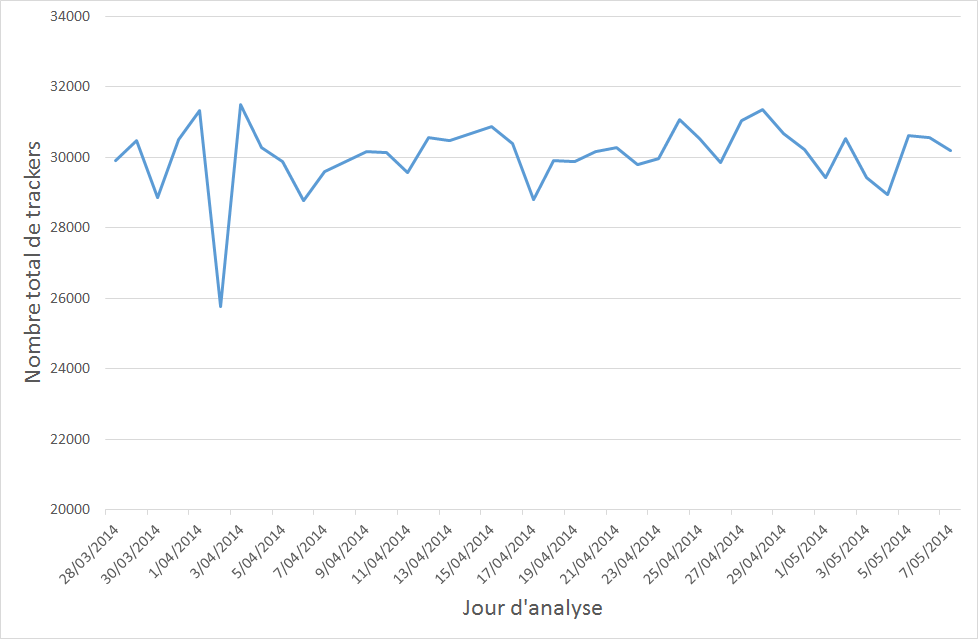
\includegraphics[scale=.8]{graphiques/Exp1_parser_total_trackers.png}
	\caption{\label{Exp1_parser_total_trackers}Nombre total de trackers sur l'ensemble de l'analyse}.
\end{figure}

\section{Expérience 2 : étude ponctuelle}
Cette expérience a été lancée de manière ponctuelle afin d'établir une image des sites à un instant donnée. Elle permet aussi de constituer la base de référence pour la comparaison des extensions.
\newline

Le \textit{crawler} a été lancé avec les paramètres suivants :
\begin{itemize}
	\item les sites visités sont issus du TOP Alexa du 16 mai 2014
	\item l'intervalle sélectionné concerne les 1000 premiers sites
	\item 3 tentatives maximum ont été autorisées par site
	\item Firefox était redémarré tous les 50 sites
	\item Firefox était dépourvu de toute extension (autre que Firebug et NetExport)
	\newline
\end{itemize}
Les 36 sites suivants ont été en échec, ce qui signifie qu'aucun fichier HTTP Archive n'a été généré pour eux :
\begin{multicols}{3}
\begin{itemize}
  \item 39.net
  \item aili.com
  \item baomihua.com
  \item bitauto.com
  \item caijing.com.cn
  \item china.com
  \item csdn.net
  \item enet.com.cn
  \item gazeta.ru
  \item gmw.cn
  \item hao123.com
  \item heise.de
  \item howstuffworks.com
  \item ifeng.com
  \item ileehoo.com
  \item justdial.com
  \item kdnet.net
  \item lady8844.com
  \item microsoftonline.com
  \item moz.com
  \item online.sh.cn
  \item onlinesbi.com
  \item opensiteexplorer.org
  \item pchome.net
  \item people.com.cn
  \item pinimg.com
  \item qq.com
  \item secureserver.net
  \item sina.com.cn
  \item sohu.com
  \item tudou.com
  \item twimg.com
  \item yesky.com
  \item yoka.com
  \item youku.com
  \item zing.vn
\end{itemize}
\end{multicols}

Ces sites ne seront par conséquent pas analysés dans cette expérience.
\newline

Par ailleurs, 78 sites ont subi au moins un timeout mais ils ne seront pas listés ici. Notez que si ces sites ont rencontré 3 timeouts consécutifs, ils sont présents dans la liste des sites en échec (ci-dessus).
\newline

Le \textit{parser} a été lancé avec le paramètre suivant :
\begin{itemize}
	\item la base de données Ghostery est la version 300
	\newline
\end{itemize}

Le \textit{parser} n'a pas été en mesure d'ouvrir les fichiers suivants :
\begin{multicols}{2}
\begin{itemize}
  \item 9gag.com.har
  \item accounts.google.com-2.har
  \item mashable.com.har
  \item website-unavailable.com-1.har
  \item www.babytree.com.har
  \item www.deezer.com.har
  \item www.gamespot.com.har
  \item www.gmail.com.har
  \item www.pixiv.net.har
  \item www.thefreedictionary.com.har
  \item www.theverge.com-1.har
  \item www.wikihow.com.har
  \item www.wix.com.har
\end{itemize}
\end{multicols}

Ces sites ne seront par conséquent pas analysés dans cette expérience.
\newline

Les critères retenus pour la classification des trackers sont les suivants :
\begin{itemize}
	\item les URL détectées comme trackers par la base de données Ghostery
	\item les réponses HTTP d'un domaine tiers qui créent un cookie
	\item les requêtes vers un domaine tiers de fichiers JavaScript avec des paramètres
	\item les requêtes de fichiers Flash
	\item les pixels de traçage
	\item les requêtes vers un domaine tiers dont l'URL contient des paramètres
	\newline
\end{itemize}

\subsection{Carte des trackers détectés}
La répartition des trackers par catégorie est disponible à la \autoref{exp_normal_detailed}. Comme on peut le constater, la majorité des trackers détectés le sont par Ghostery. Ceci est normal car c'est le premier critère appliqué. En deuxième position, viennent les URL appelées avec des paramètres et en troisième position, les cookies créés dans les réponses HTTP de domaines tiers.

\begin{figure}[h]
	\centering
	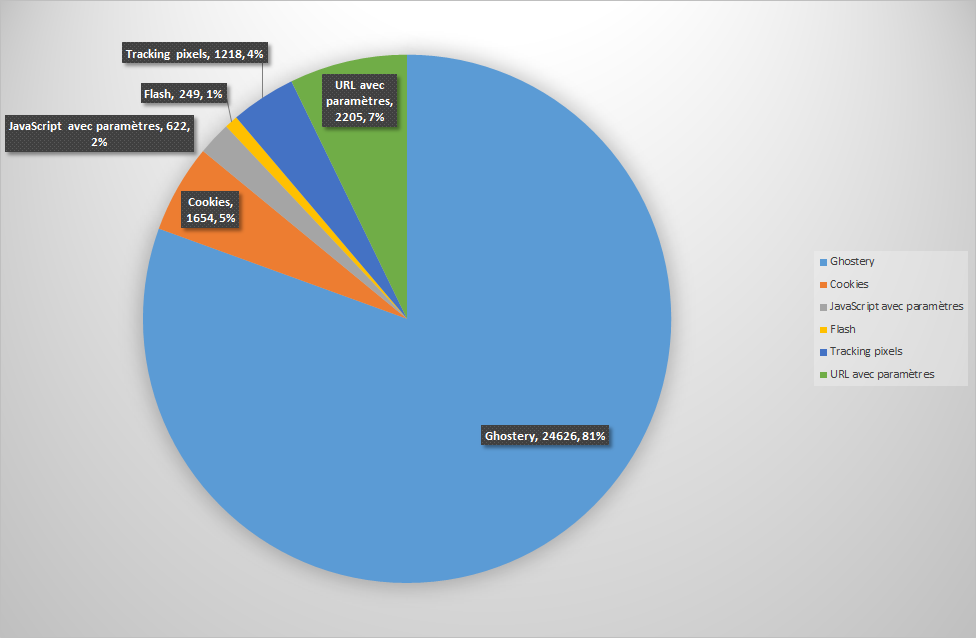
\includegraphics[scale=.60]{Analyses_graphiques/Images/Normal_detailed.png}
	\caption{\label{exp_normal_detailed}Répartition des trackers par catégorie}.
\end{figure}

Lorsqu'une ressource est détectée comme étant un tracker par Ghostery, le \textit{parser} regarde le type de cette ressource. Les résultats sont visibles à la \autoref{exp_normal_ghostery}. Ils montrent que le premier type de trackers est le \textit{gif}. La deuxième position est occupée par le JavaScript (si on rassemble \textit{text/javascript}, \textit{application/x-javascript} et \textit{application/javascript}).
\begin{figure}[h]
	\centering
	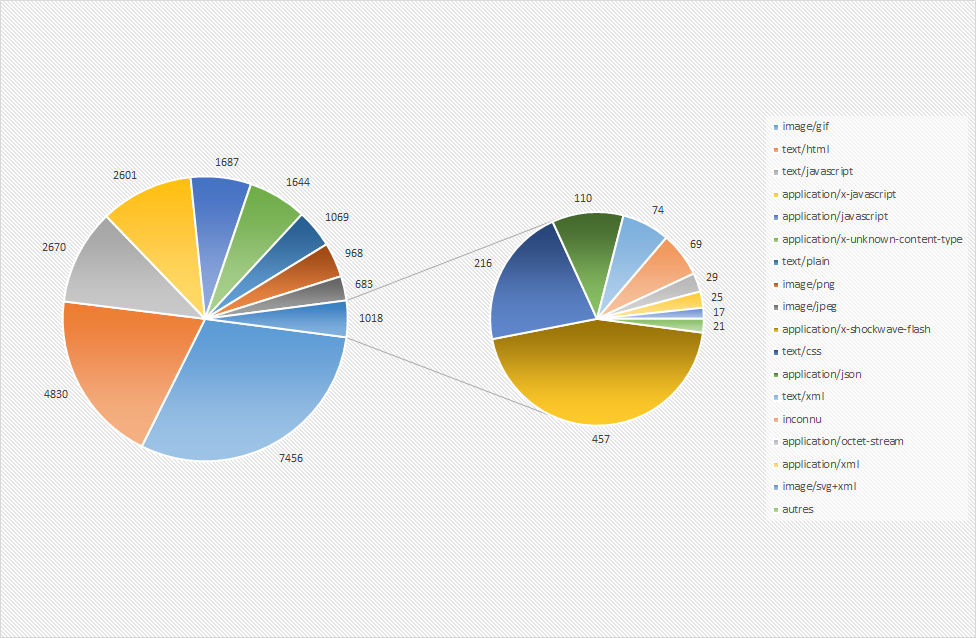
\includegraphics[scale=.60]{Analyses_graphiques/Images/Normal_ghostery.png}
	\caption{\label{exp_normal_ghostery}Répartition des types de trackers détectés par Ghostery}.
\end{figure}

\subsection{Sites renfermant le plus de trackers détectés}
Le TOP 10 des sites en nombre de trackers détectés sont :
\begin{itemize}
	\item drudgereport.com : 347 trackers dont 326 avec Ghostery\\(blog d'information sur Internet)
	\item www.hongkiat.com : 344 trackers dont 318 avec Ghostery\\(blog d'information sur le design Web)
	\item www.primewire.ag : 286 trackers dont 273 avec Ghostery\\(site de streaming audio et vidéo)
	\item www.theblaze.com : 262 trackers dont 235 avec Ghostery\\(site d'information)
	\item photobucket.com : 240 trackers dont 234 avec Ghostery\\(hébergeur d'images)
	\item slickdeals.net : 237 trackers dont 211 avec Ghostery\\(portail regroupant des coupons de réduction)
	\item www.jeuxvideo.com : 226 trackers dont 202 avec Ghostery\\(portail sur les jeux vidéos)
	\item www.engadget.com : 216 trackers dont 201 avec Ghostery\\(portail sur la technologie)
	\item www.linternaute.com : 212 trackers dont 200 avec Ghostery\\(site d'actualités)
	\item www.gap.com : 206 trackers dont 193 avec Ghostery\\(site de vente de vêtements)
	\newline
\end{itemize}

\subsection{Organisations déployant le plus de trackers}
En ne considérant que les trackers détectés par Ghostery, voici la liste des organisations dont le plus de trackers ont été détectés dans cette analyse.
\newline

Sur un total de 24626 trackers :
\begin{itemize}
  \item 2562 sont de DoubleClick
  \item 1379 sont de AppNexus
  \item 949 sont de Google Analytics
  \item 675 sont de Google Adsense
  \item 574 sont de Rubicon
  \item 534 sont de Turn
  \item 441 sont de ScoreCard Research Beacon
  \item 347 sont de MediaMath
  \item 332 sont de Lotame
  \item 326 sont de OpenX
  \newline
\end{itemize}

Quand on sait que DoubleClick appartient à Google, cela fait 4186 trackers provenant de Google qui ont été détectés. Cela représente 17\% des trackers détectés au total par la base de données Ghostery.
